\begin{figure*}[t]
\centering
\noindent\textbf{Eleven physical task cases organized into four functional families}
\hfill{\textcolor{TraceSlate}{\small 30/30 required conditions}}
\par\vspace{4pt}
\begin{minipage}[t]{0.242\textwidth}
\centering
\textbf{Reach and dynamic motion}\par\vspace{2pt}
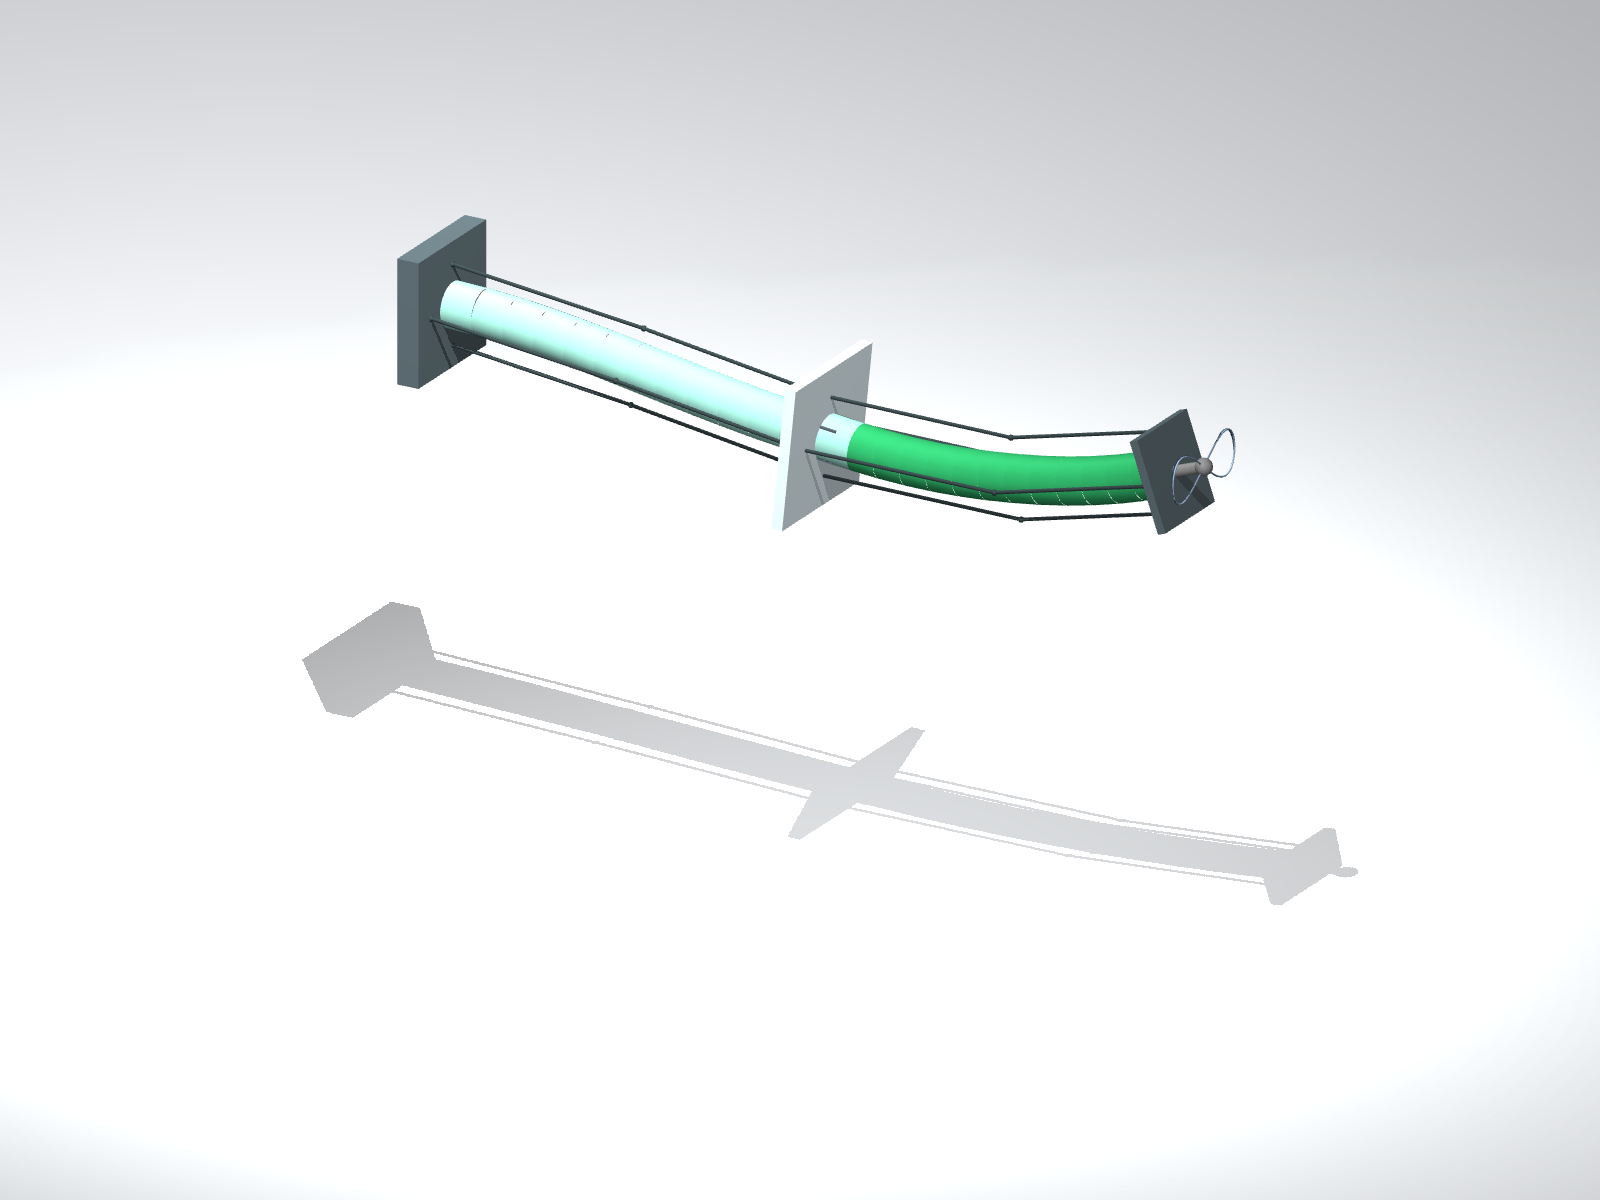
\includegraphics[width=.96\linewidth,height=.78in,keepaspectratio]{figures/native/t04_final.png}
\par{\scriptsize Representative native robot state}
\vspace{3pt}\hrule\vspace{3pt}
\raggedright\scriptsize
\textbf{T01} Multi-target reach-and-hold\\[-1pt]
\hspace*{1em}3/3 · Hold 9.906 mm\\[2pt]
\textbf{T02} Load-conditioned hold\\[-1pt]
\hspace*{1em}3/3 · Hold 9.897 mm\\[2pt]
\textbf{T03} Fast target reaching\\[-1pt]
\hspace*{1em}1/1 · Terminal/hold 2.110/2.663 mm\\[2pt]
\textbf{T04} Figure-eight tracking\\[-1pt]
\hspace*{1em}1/1 · RMSE 0.688 mm
\end{minipage}\hfill
\begin{minipage}[t]{0.242\textwidth}
\centering
\textbf{Pose and contact interaction}\par\vspace{2pt}
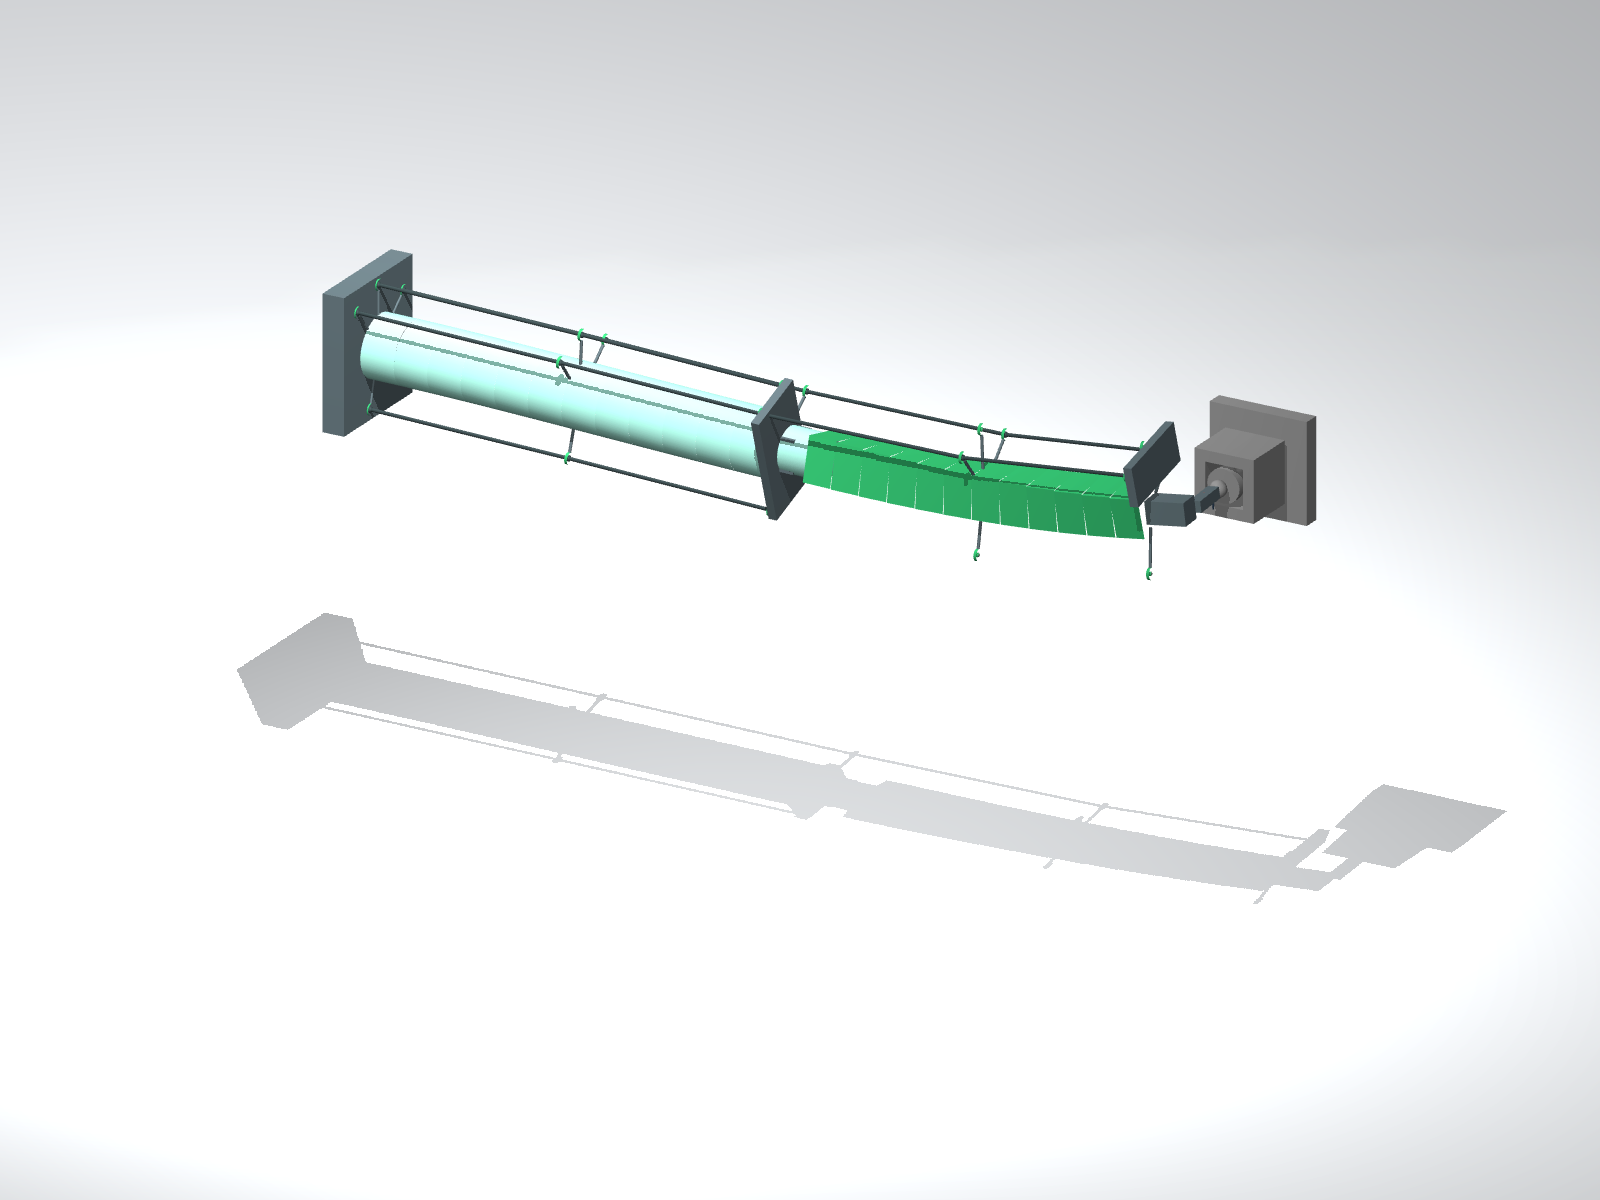
\includegraphics[width=.96\linewidth,height=.78in,keepaspectratio]{figures/native/t09_hold.png}
\par{\scriptsize Representative native robot state}
\vspace{3pt}\hrule\vspace{3pt}
\raggedright\scriptsize
\textbf{T05} Position and tool-axis alignment\\[-1pt]
\hspace*{1em}1/1 · 7.458 mm / 0.0518 rad\\[2pt]
\textbf{T06} Loaded time-indexed pose scan\\[-1pt]
\hspace*{1em}1/1 · 11.820 mm / 0.1104 rad\\[2pt]
\textbf{T09} Guided spring-button contact\\[-1pt]
\hspace*{1em}1/1 · 0.0528 mm / 0.00247 N
\end{minipage}\hfill
\begin{minipage}[t]{0.242\textwidth}
\centering
\textbf{Shared morphology and control}\par\vspace{2pt}
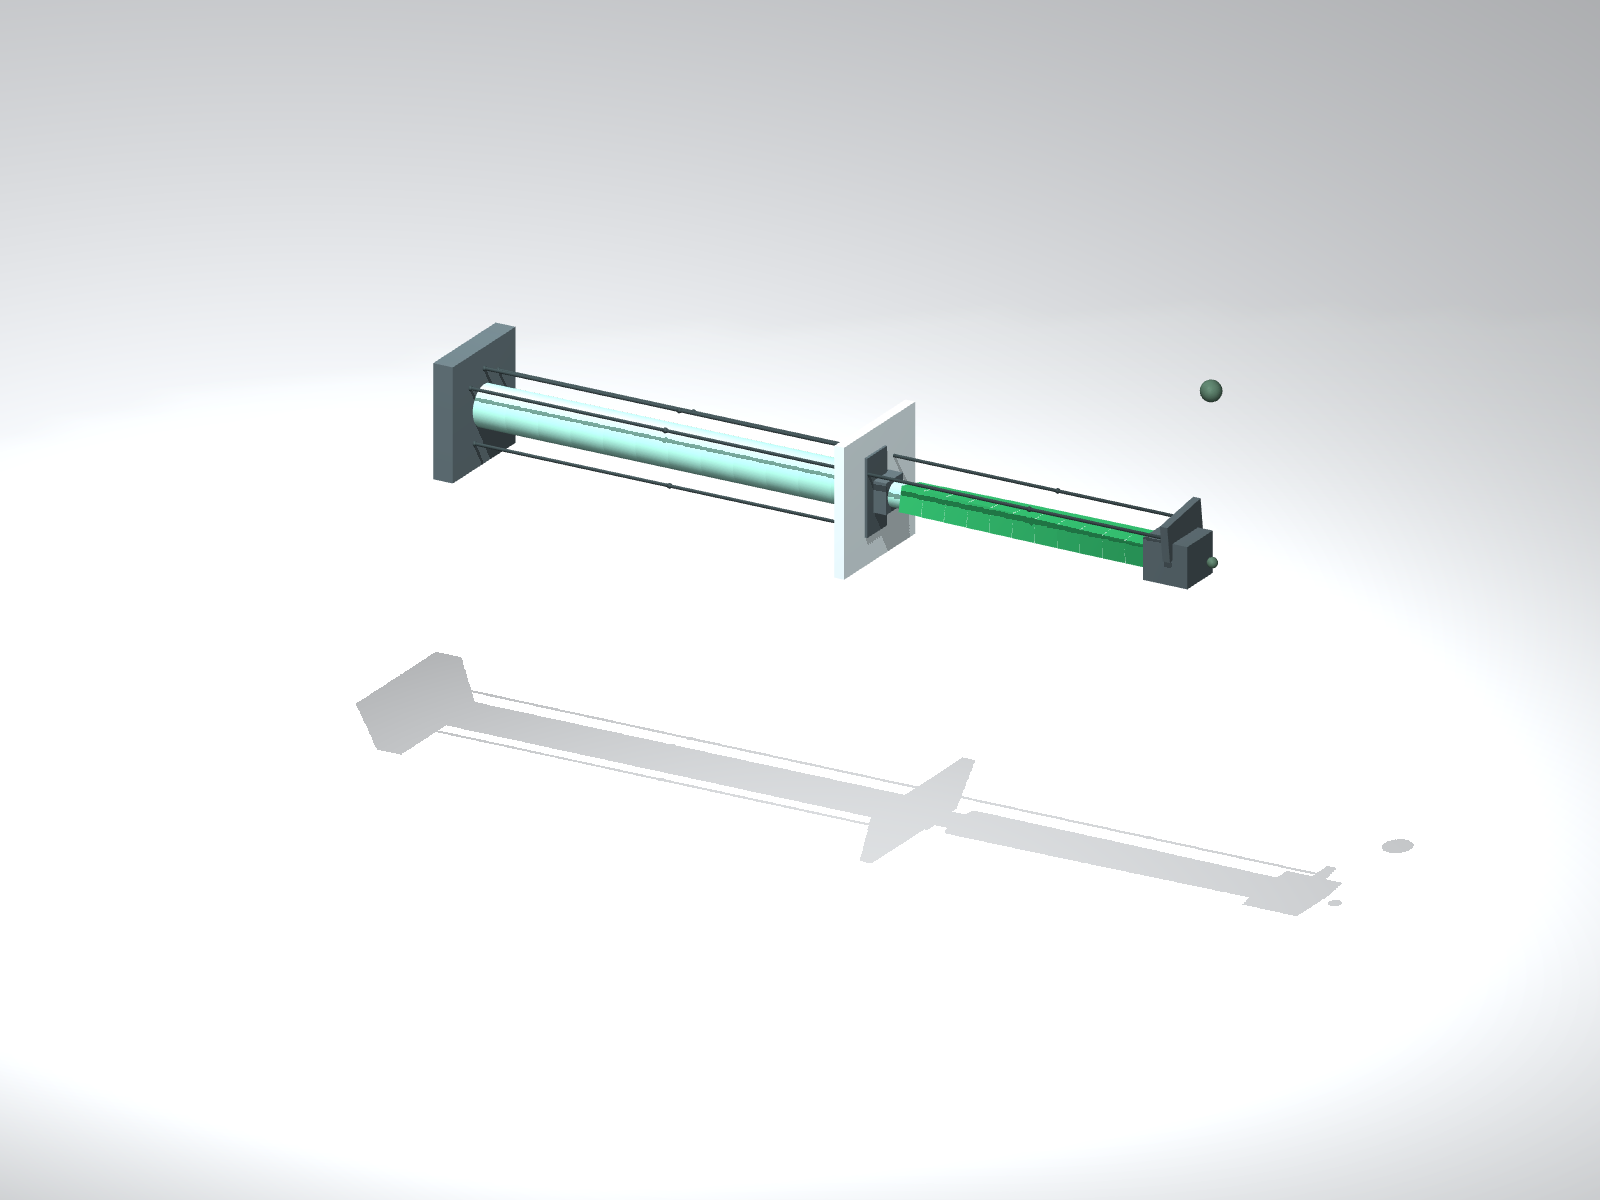
\includegraphics[width=.96\linewidth,height=.78in,keepaspectratio]{figures/native/t07_round_root.png}
\par{\scriptsize Representative native robot state}
\vspace{3pt}\hrule\vspace{3pt}
\raggedright\scriptsize
\textbf{T07} Shared-morphology multi-task design\\[-1pt]
\hspace*{1em}4/4 · Position 7.920 mm; axis 0.0518 rad\\[2pt]
\textbf{T10} Impact-recovery control\\[-1pt]
\hspace*{1em}3/3 · Final hold error 4.131 mm
\end{minipage}\hfill
\begin{minipage}[t]{0.242\textwidth}
\centering
\textbf{Passive mechanics}\par\vspace{2pt}
\begin{tikzpicture}[x=1cm,y=1cm]
\draw[TraceNavy,line width=2.2pt] (0.82,0.08) -- (0.82,0.88);
\draw[TraceTeal,line width=0.8pt] (0.55,0.08) .. controls (0.62,0.36) and (0.98,0.58) .. (1.08,0.88);
\draw[TraceSlate,line width=0.8pt] (1.09,0.08) .. controls (1.02,0.36) and (0.66,0.58) .. (0.56,0.88);
\foreach \y in {0.22,0.42,0.62,0.82}
  \draw[fill=white,draw=TraceSlate,line width=0.55pt] (0.69,\y) rectangle (0.95,\y+0.035);
\draw[fill=TraceNavy] (0.66,0.02) rectangle (0.98,0.12);
\end{tikzpicture}
\par{\scriptsize Passive tendon-constrained schematic}
\vspace{3pt}\hrule\vspace{3pt}
\raggedright\scriptsize
\textbf{T08} Passive progressive-stiffness response\\[-1pt]
\hspace*{1em}2/2 · Stiffness ratio 1.631\\[2pt]
\textbf{PHS-2D} Passive tendon-constrained compliance\\[-1pt]
\hspace*{1em}10/10 · Maximum tip/point ratio 0.1538
\end{minipage}
\caption{Functional task-space overview of the eleven-task physical portfolio. Each family is illustrated by a representative native robot state or a passive-mechanism schematic and lists its constituent tasks, required-condition completion, and principal task-specific outcome. Metrics retain their native physical units and are not averaged across task families.}
\label{fig:task-portfolio}
\end{figure*}
